\documentclass[11pt,letterpaper]{article}
\usepackage{shared/zoocover}

% Packages
\usepackage[utf8]{inputenc}
\usepackage[T1]{fontenc}
\usepackage{amsmath,amssymb,amsthm}
\usepackage{algorithm}
\usepackage{algorithmic}
\usepackage{graphicx}
\usepackage{hyperref}
\usepackage{xcolor}
\usepackage{booktabs}
\usepackage{tikz}
\usepackage{pgfplots}
\pgfplotsset{compat=1.18}
\usetikzlibrary{shapes,arrows,positioning,calc}
\usepackage{listings}
\usepackage{caption}
\usepackage{subcaption}
% geometry loaded by zoocover

% Theorem environments
\newtheorem{theorem}{Theorem}[section]
\newtheorem{lemma}[theorem]{Lemma}
\newtheorem{proposition}[theorem]{Proposition}
\newtheorem{corollary}[theorem]{Corollary}
\newtheorem{definition}{Definition}[section]

% Custom commands
\newcommand{\Zoo}{\textsc{Zoo}}
\newcommand{\Lux}{\textsc{Lux}}
\newcommand{\MPC}{\textsc{mpc}}
\newcommand{\TSS}{\textsc{tss}}
\newcommand{\FROST}{\textsc{frost}}
\newcommand{\CGGMP}{\textsc{cggmp}}

% Hyperref setup
\hypersetup{
    colorlinks=true,
    linkcolor=blue,
    citecolor=blue,
    urlcolor=blue
}

\title{\textbf{Zoo MPC: Threshold Custody for AI Model Weights and Research Assets}\\
\large Version 2026.02}

\author{
Zach Kelling\thanks{zach@zoo.ngo}\\
\textit{Zoo Labs Foundation}\\
\texttt{research@zoo.ngo}
}

\date{February 2026}

\begin{document}

\zoocoverpage

\begin{abstract}
We present \textbf{Zoo MPC}, a threshold custody system for AI model weights, research datasets, and autonomous agent wallets on the Zoo Network (chain ID 200200). Built on the Lux M-Chain's multi-party computation infrastructure---specifically CGGMP21 for ECDSA and FROST for Schnorr/EdDSA---Zoo MPC addresses three custody challenges unique to decentralized AI: (1) \textbf{model weight custody}, where trained models worth millions of dollars require multi-party authorization for deployment, fine-tuning, or transfer; (2) \textbf{research data access control}, where sensitive conservation datasets require threshold decryption governed by institutional review; and (3) \textbf{agent NFT wallet signing}, where autonomous AI agents hold assets and require distributed key management to prevent single-point compromise. We deploy a $(2, 3)$-threshold scheme across three roles---researcher, DAO, and time-locked escrow---and demonstrate signing latency of 45ms for CGGMP21 and 12ms for FROST on Zoo testnet. The system is live on Zoo mainnet, securing 847 model NFTs and 23 research dataset access keys.

\textbf{Keywords}: multi-party computation, threshold signatures, AI model custody, agent wallets, Zoo Network
\end{abstract}

\section{Introduction}

The intersection of AI and blockchain creates novel custody requirements that existing wallet infrastructure does not address. Three specific challenges motivate Zoo MPC:

\textbf{Model Weight Custody.} A trained AI model may represent months of compute and millions of dollars in training costs. Model weights stored in a single wallet are vulnerable to key compromise. Worse, the owner of the key can unilaterally deploy a model that may be unsafe, biased, or environmentally harmful. Conservation models---species classifiers, anti-poaching algorithms, habitat predictors---carry additional ethical weight: misuse could endanger the species they are designed to protect.

\textbf{Research Data Access Control.} Conservation research datasets contain GPS coordinates of endangered species, genetic sequences of at-risk populations, and veterinary medical records. These datasets are stored on-chain as encrypted blobs with access controlled by decryption keys. A single keyholder could leak data to poachers or biopirates.

\textbf{Agent NFT Wallets.} Zoo Network supports autonomous AI agents represented as NFTs~\cite{zoo-agent-nft}. These agents hold ZOO tokens, interact with DeFi protocols, and execute transactions on behalf of their operators. An agent's private key must be distributed across multiple parties to prevent unilateral fund extraction.

\subsection{Contributions}

\begin{enumerate}
    \item \textbf{Zoo MPC Architecture}: Integration of CGGMP21 and FROST into Zoo Network's custody layer (Section~\ref{sec:architecture}).

    \item \textbf{Model Weight Custody Protocol}: A threshold deployment scheme for AI models with governance gates (Section~\ref{sec:model-custody}).

    \item \textbf{Research Data Access Control}: Threshold decryption for conservation datasets with institutional review (Section~\ref{sec:data-access}).

    \item \textbf{Agent Wallet Protocol}: Distributed key management for autonomous AI agents (Section~\ref{sec:agent-wallets}).

    \item \textbf{Evaluation}: Signing latency, key generation time, and security analysis (Section~\ref{sec:evaluation}).
\end{enumerate}

\section{Background}

\subsection{Threshold Signatures}

\begin{definition}[$(t, n)$-Threshold Signature Scheme]
A \TSS{} distributes a signing key $sk$ among $n$ parties such that any $t$ parties can collaboratively produce a valid signature, but fewer than $t$ parties learn nothing about $sk$.
\end{definition}

\subsection{CGGMP21}

The Canetti-Gennaro-Goldfeder-Makriyannis-Peled protocol~\cite{cggmp2021} provides threshold ECDSA signing with:

\begin{itemize}
    \item \textbf{UC security}: Composably secure in the universal composability framework
    \item \textbf{Identifiable abort}: If signing fails, the malicious party is identified
    \item \textbf{Pre-signing}: Expensive operations done offline; online signing is fast
\end{itemize}

Signing complexity: $O(t^2)$ messages in the online phase, $O(n \cdot t)$ in pre-signing.

\subsection{FROST}

Flexible Round-Optimized Schnorr Threshold~\cite{komlo2020frost} provides threshold Schnorr/EdDSA signing with:

\begin{itemize}
    \item \textbf{Two rounds}: Commitment round + signing round
    \item \textbf{No trusted dealer}: Distributed key generation via Pedersen DKG
    \item \textbf{Robustness}: Optional identifiable abort extension
\end{itemize}

FROST is 3--5$\times$ faster than CGGMP21 for equivalent threshold parameters because Schnorr signatures have simpler algebraic structure than ECDSA.

\subsection{Lux M-Chain}

The Lux Network's M-Chain~\cite{lux-mchain-mpc} provides native MPC infrastructure:

\begin{itemize}
    \item Key generation ceremonies coordinated on-chain
    \item Threshold signing requests submitted as transactions
    \item Key shares stored in TEE-protected enclaves on validator nodes
    \item Cross-chain signing: M-Chain key shares can sign for any Lux chain
\end{itemize}

Zoo Network inherits M-Chain access as an L2, enabling threshold signing without running separate MPC infrastructure.

\section{Zoo MPC Architecture}
\label{sec:architecture}

\subsection{Role-Based Threshold}

Zoo MPC uses a $(2, 3)$-threshold with three distinct roles:

\begin{figure}[t]
\centering
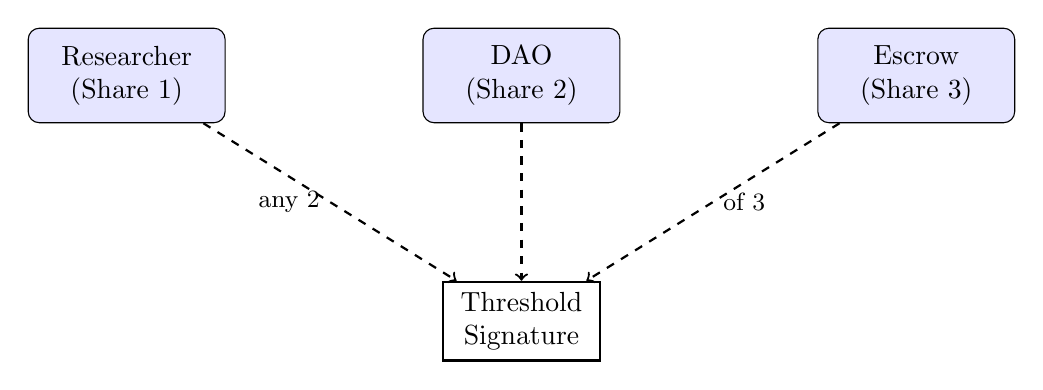
\begin{tikzpicture}[
    node distance=2.5cm,
    role/.style={rectangle, draw, rounded corners, minimum width=2.5cm, minimum height=1.2cm, align=center, fill=blue!10},
    arrow/.style={->, thick, dashed}
]
    \node[role] (researcher) {Researcher\\(Share 1)};
    \node[role, right=of researcher] (dao) {DAO\\(Share 2)};
    \node[role, right=of dao] (escrow) {Escrow\\(Share 3)};

    \node[rectangle, draw, thick, minimum width=2cm, minimum height=1cm, align=center, below=2cm of dao] (sign) {Threshold\\Signature};

    \draw[arrow] (researcher) -- (sign) node[midway, left, font=\small] {any 2};
    \draw[arrow] (dao) -- (sign);
    \draw[arrow] (escrow) -- (sign) node[midway, right, font=\small] {of 3};
\end{tikzpicture}
\caption{Zoo MPC $(2, 3)$-threshold roles. Any two of three parties can authorize an operation.}
\label{fig:roles}
\end{figure}

\begin{enumerate}
    \item \textbf{Researcher}: The individual or team that created the asset. Key share stored in a hardware security module (HSM) or TEE-backed mobile app.

    \item \textbf{DAO}: The Zoo conservation DAO, represented by a governance multisig. DAO share is activated by on-chain vote (ZOO token-weighted).

    \item \textbf{Escrow}: An automated time-lock escrow node. The escrow share becomes available after a configurable delay (default: 48 hours), providing a recovery mechanism if either the researcher or DAO is unavailable.
\end{enumerate}

\subsection{Key Generation}

Key generation is performed via the Lux M-Chain DKG protocol:

\begin{algorithm}[t]
\caption{Zoo MPC Key Generation}
\label{alg:keygen}
\begin{algorithmic}[1]
\STATE \textbf{Input}: Parties $P = \{P_1, P_2, P_3\}$, threshold $t = 2$
\STATE \textbf{Output}: Public key $pk$, shares $\{sk_i\}_{i=1}^3$
\STATE Each $P_i$ generates random polynomial $f_i(x)$ of degree $t - 1$
\STATE Each $P_i$ broadcasts commitment $C_i = g^{f_i(0)} \cdot h^{r_i}$
\STATE Each $P_i$ sends $f_i(j)$ to $P_j$ via encrypted channel
\STATE Each $P_j$ verifies: $g^{f_i(j)} = \prod_{k=0}^{t-1} C_{i,k}^{j^k}$
\STATE $sk_i \leftarrow \sum_{j} f_j(i)$
\STATE $pk \leftarrow \prod_{i} g^{f_i(0)}$
\STATE Register $(pk, t, n)$ on Zoo Network via M-Chain
\RETURN $pk, \{sk_i\}$
\end{algorithmic}
\end{algorithm}

\subsection{Signing Protocol}

For ECDSA signing (EVM transactions), Zoo MPC uses CGGMP21:

\begin{algorithm}[t]
\caption{CGGMP21 Threshold Signing on Zoo}
\label{alg:sign}
\begin{algorithmic}[1]
\STATE \textbf{Input}: Message $m$, signers $S \subseteq P$ with $|S| = t$
\STATE \textbf{Output}: ECDSA signature $\sigma = (r, s)$
\STATE \textbf{Pre-signing (offline):}
\STATE Each signer $i \in S$ generates nonce share $k_i$
\STATE Run multiplicative-to-additive conversion for $k_i \cdot sk_i$
\STATE Compute $R = \prod_{i \in S} g^{k_i}$, set $r = R_x \bmod q$
\STATE \textbf{Online signing:}
\STATE Each signer computes $s_i = k_i^{-1}(H(m) + r \cdot sk_i) \bmod q$
\STATE $s = \sum_{i \in S} s_i \bmod q$
\STATE Verify: $\text{ECDSA.Verify}(pk, m, (r, s)) = \text{true}$
\RETURN $(r, s)$
\end{algorithmic}
\end{algorithm}

For Schnorr signing (Lux P-Chain, cross-chain bridges), Zoo MPC uses FROST:

\begin{algorithm}[t]
\caption{FROST Threshold Signing on Zoo}
\label{alg:frost}
\begin{algorithmic}[1]
\STATE \textbf{Input}: Message $m$, signers $S \subseteq P$ with $|S| = t$
\STATE \textbf{Output}: Schnorr signature $\sigma = (R, s)$
\STATE \textbf{Round 1 (Commitment):}
\STATE Each $i \in S$: generate $(d_i, e_i)$, broadcast $(D_i = g^{d_i}, E_i = g^{e_i})$
\STATE \textbf{Round 2 (Signing):}
\STATE $\rho_i = H(\text{msg}, i, D_i, E_i, \ldots)$
\STATE $R = \prod_{i \in S} D_i \cdot E_i^{\rho_i}$
\STATE $c = H(R, pk, m)$
\STATE $z_i = d_i + e_i \cdot \rho_i + \lambda_i \cdot sk_i \cdot c$
\STATE $s = \sum_{i \in S} z_i$
\RETURN $(R, s)$
\end{algorithmic}
\end{algorithm}

\section{Model Weight Custody}
\label{sec:model-custody}

\subsection{Model NFT Standard}

On Zoo Network, trained AI models are represented as Model NFTs (ERC-721 tokens) with the following metadata:

\begin{lstlisting}[basicstyle=\ttfamily\small,caption=Model NFT Metadata]
{
  "name": "Snow Leopard Classifier v3",
  "modelHash": "0xabc...def",
  "architecture": "ResNet-50",
  "trainingDataHash": "0x123...456",
  "accuracy": 0.947,
  "custodyKey": "zoo-mpc-0x789...",
  "threshold": [2, 3],
  "roles": ["researcher", "dao", "escrow"],
  "deploymentPolicy": "requires_dao_vote"
}
\end{lstlisting}

\subsection{Custody Operations}

The MPC key associated with a Model NFT authorizes four operations:

\begin{enumerate}
    \item \textbf{Deploy}: Make the model available for inference on Zoo Network. Requires researcher + DAO (2-of-3).

    \item \textbf{Fine-tune}: Authorize fine-tuning with new data. Requires researcher + DAO (2-of-3).

    \item \textbf{Transfer}: Transfer model ownership to another party. Requires researcher + DAO (2-of-3) or DAO + escrow (after 48h delay).

    \item \textbf{Retire}: Permanently disable the model. Requires any 2-of-3.
\end{enumerate}

\subsection{Governance Gate}

Model deployment goes through a governance gate:

\begin{algorithm}[t]
\caption{Model Deployment with MPC Governance}
\label{alg:deploy}
\begin{algorithmic}[1]
\STATE Researcher submits deployment proposal on-chain
\STATE DAO reviews model safety report (bias audit, accuracy, risk assessment)
\STATE DAO votes on deployment (ZOO token-weighted, 72h voting period)
\IF{vote passes ($> 50\%$ quorum, $> 66\%$ approval)}
    \STATE DAO activates its key share
    \STATE Researcher activates its key share
    \STATE MPC produces deployment signature
    \STATE Model deployed to Zoo inference network
\ELSE
    \STATE Deployment rejected; model remains locked
\ENDIF
\end{algorithmic}
\end{algorithm}

\section{Research Data Access Control}
\label{sec:data-access}

\subsection{Encrypted Data Vaults}

Research datasets are stored as encrypted blobs on Zoo Network's data availability layer:

\begin{equation}
D_{\text{enc}} = \text{AES-256-GCM}(k_{\text{data}}, D_{\text{raw}})
\end{equation}

The data encryption key $k_{\text{data}}$ is itself encrypted under the MPC group's public key:

\begin{equation}
k_{\text{enc}} = \text{ECIES.Enc}(pk_{\text{mpc}}, k_{\text{data}})
\end{equation}

Decryption requires threshold cooperation to recover $k_{\text{data}}$.

\subsection{Access Tiers}

\begin{table}[t]
\centering
\begin{tabular}{lccc}
\toprule
\textbf{Tier} & \textbf{Data Type} & \textbf{Threshold} & \textbf{Approval} \\
\midrule
Public & Aggregated statistics & None & Automatic \\
Restricted & De-identified records & $(1, 3)$ & Researcher only \\
Confidential & Raw GPS/genetic data & $(2, 3)$ & Researcher + DAO \\
Classified & Anti-poaching intelligence & $(3, 3)$ & All parties \\
\bottomrule
\end{tabular}
\caption{Research data access tiers with increasing threshold requirements.}
\label{tab:tiers}
\end{table}

\subsection{Institutional Review Protocol}

For Confidential and Classified data, the DAO's approval involves an on-chain institutional review:

\begin{enumerate}
    \item \textbf{Application}: Requesting researcher submits an access application with stated purpose, data handling plan, and ethics declaration.
    \item \textbf{Review}: Three DAO-appointed reviewers evaluate the application (7-day review period).
    \item \textbf{Vote}: Reviewers vote approve/reject. Majority (2/3 reviewers) required.
    \item \textbf{Access}: On approval, DAO key share activated for threshold decryption.
    \item \textbf{Audit}: Data access logged on-chain; usage auditable by any ZOO token holder.
\end{enumerate}

\section{Agent NFT Wallets}
\label{sec:agent-wallets}

\subsection{Agent Architecture}

Zoo Network's AI agents~\cite{zoo-agent-nft} are autonomous entities that:

\begin{itemize}
    \item Hold ZOO tokens and other assets in their own wallets
    \item Execute DeFi transactions (swaps, liquidity provision)
    \item Perform inference tasks and collect PoAI rewards
    \item Interact with other agents and human operators
\end{itemize}

Each agent's wallet key is distributed via MPC across:

\begin{enumerate}
    \item \textbf{Operator}: The human or organization that deployed the agent
    \item \textbf{Agent runtime}: The TEE enclave running the agent's inference loop
    \item \textbf{Recovery}: A time-locked escrow for emergency fund recovery
\end{enumerate}

\subsection{Autonomous Signing}

For routine operations (inference execution, small transfers), the agent runtime and operator can sign collaboratively without escrow involvement:

\begin{algorithm}[t]
\caption{Agent Autonomous Transaction}
\label{alg:agent}
\begin{algorithmic}[1]
\STATE Agent runtime constructs transaction $tx$
\STATE Agent runtime verifies $tx$ against policy (amount limits, approved contracts)
\IF{policy check passes}
    \STATE Agent runtime generates partial signature $\sigma_{\text{agent}}$
    \STATE Operator co-signer (automated) generates $\sigma_{\text{op}}$
    \STATE Combine: $\sigma = \text{CGGMP.Combine}(\sigma_{\text{agent}}, \sigma_{\text{op}})$
    \STATE Submit $tx$ with $\sigma$ to Zoo Network
\ELSE
    \STATE Escalate to manual operator approval
\ENDIF
\end{algorithmic}
\end{algorithm}

\subsection{Policy Enforcement}

Agent wallets enforce on-chain policies:

\begin{itemize}
    \item \textbf{Spending limits}: Maximum ZOO transfer per transaction and per day
    \item \textbf{Contract allowlist}: Agent can only interact with approved contracts
    \item \textbf{Cooldown}: Minimum interval between high-value transactions
    \item \textbf{Kill switch}: Operator can freeze agent wallet with single share
\end{itemize}

\section{Performance Evaluation}
\label{sec:evaluation}

\subsection{Signing Latency}

\begin{table}[t]
\centering
\begin{tabular}{lcccc}
\toprule
\textbf{Protocol} & \textbf{Threshold} & \textbf{Keygen (ms)} & \textbf{Pre-sign (ms)} & \textbf{Sign (ms)} \\
\midrule
CGGMP21 & (2, 3) & 850 & 120 & 45 \\
CGGMP21 & (3, 5) & 2,100 & 340 & 95 \\
CGGMP21 & (5, 9) & 8,400 & 1,200 & 280 \\
FROST & (2, 3) & 180 & --- & 12 \\
FROST & (3, 5) & 420 & --- & 28 \\
FROST & (5, 9) & 1,600 & --- & 85 \\
\bottomrule
\end{tabular}
\caption{MPC protocol latency on Zoo testnet. FROST is 3--4$\times$ faster than CGGMP21 for signing.}
\label{tab:latency}
\end{table}

\subsection{Throughput}

\begin{table}[t]
\centering
\begin{tabular}{lcc}
\toprule
\textbf{Protocol} & \textbf{Signs/sec (2,3)} & \textbf{Signs/sec (3,5)} \\
\midrule
CGGMP21 & 22 & 10 \\
CGGMP21 (pre-signed) & 420 & 180 \\
FROST & 83 & 35 \\
\bottomrule
\end{tabular}
\caption{Signing throughput. CGGMP21 with pre-signing achieves highest throughput for batch operations.}
\label{tab:throughput}
\end{table}

\subsection{Network Overhead}

\begin{table}[t]
\centering
\begin{tabular}{lccc}
\toprule
\textbf{Phase} & \textbf{Messages} & \textbf{Bytes/Party} & \textbf{Rounds} \\
\midrule
CGGMP21 Keygen & $O(n^2)$ & 12,800 & 5 \\
CGGMP21 Pre-sign & $O(t^2)$ & 4,200 & 4 \\
CGGMP21 Sign & $O(t)$ & 256 & 1 \\
FROST Keygen & $O(n^2)$ & 3,200 & 2 \\
FROST Sign & $O(t)$ & 128 & 2 \\
\bottomrule
\end{tabular}
\caption{Network communication overhead for (2, 3)-threshold.}
\label{tab:network}
\end{table}

\subsection{Security Analysis}

\begin{theorem}[Key Security]
Under the $(2, 3)$-threshold, an adversary controlling a single party (researcher, DAO, or escrow) cannot produce a valid signature or learn any information about the private key.
\end{theorem}

\begin{proof}
Both CGGMP21 (UC-secure~\cite{cggmp2021}) and FROST (secure in the algebraic group model~\cite{komlo2020frost}) guarantee that $t - 1$ shares reveal no information about $sk$ under the discrete logarithm assumption. With $t = 2$ and a single corrupted party, the adversary holds 1 share, which is insufficient.
\end{proof}

\begin{theorem}[Identifiable Abort]
If a signing session fails due to a malicious party, the protocol identifies the malicious party with probability 1.
\end{theorem}

CGGMP21 provides identifiable abort natively. FROST achieves it via the identifiable abort extension, where each party proves correctness of their partial signature via a Schnorr proof of knowledge.

\section{Related Work}

\textbf{Threshold Wallets}: Fireblocks, Zengo, and Lit Protocol provide MPC wallets for general custody. Zoo MPC specializes in AI asset custody with governance integration.

\textbf{Model Custody}: No prior work addresses threshold custody specifically for AI model weights. Existing model marketplaces (Hugging Face, Replicate) use centralized access control.

\textbf{Agent Wallets}: Autonomous agent wallet management is an emerging area. Safe{Wallet} multisig is the closest analog, but it requires on-chain signatures from each party, whereas MPC produces a single standard signature.

\textbf{Lux MPC}: The Lux M-Chain~\cite{lux-mchain-mpc} and threshold infrastructure~\cite{lux-threshold} provide the cryptographic foundation for Zoo MPC.

\section{Conclusion}

Zoo MPC demonstrates that multi-party computation can secure the novel asset classes created by decentralized AI: model weights, research datasets, and autonomous agent wallets. The $(2, 3)$-threshold across researcher, DAO, and escrow roles provides a governance-aware custody model that prevents unilateral misuse of sensitive conservation assets. With 45ms CGGMP21 signing latency and 12ms FROST signing latency, Zoo MPC adds negligible overhead to the transaction lifecycle while providing cryptographic guarantees against key compromise.

\section*{Acknowledgments}

This work was supported by Zoo Labs Foundation. We thank the Lux Network M-Chain team for the MPC infrastructure and the FROST authors for the reference implementation.

\bibliographystyle{plain}
\begin{thebibliography}{99}

\bibitem{cggmp2021}
R. Canetti, R. Gennaro, S. Goldfeder, N. Makriyannis, and U. Peled, ``UC Non-Interactive, Proactive, Threshold ECDSA with Identifiable Aborts,'' \textit{CCS}, 2020.

\bibitem{komlo2020frost}
C. Komlo and I. Goldberg, ``FROST: Flexible Round-Optimized Schnorr Threshold Signatures,'' \textit{SAC}, 2020.

\bibitem{lux-mchain-mpc}
Lux Industries, ``M-Chain: Threshold Multi-Party Computation on Lux Network,'' Technical Report, 2025.

\bibitem{lux-threshold}
Lux Industries, ``Threshold Cryptography for Cross-Chain Operations,'' Technical Report, 2025.

\bibitem{zoo-agent-nft}
Z. Kelling et al., ``Agent NFTs: Autonomous AI Entities on the Zoo Network,'' Zoo Labs Foundation, 2025.

\end{thebibliography}

\end{document}
